% Created by tikzDevice version 0.12.6 on 2024-08-01 12:50:15
% !TEX encoding = UTF-8 Unicode
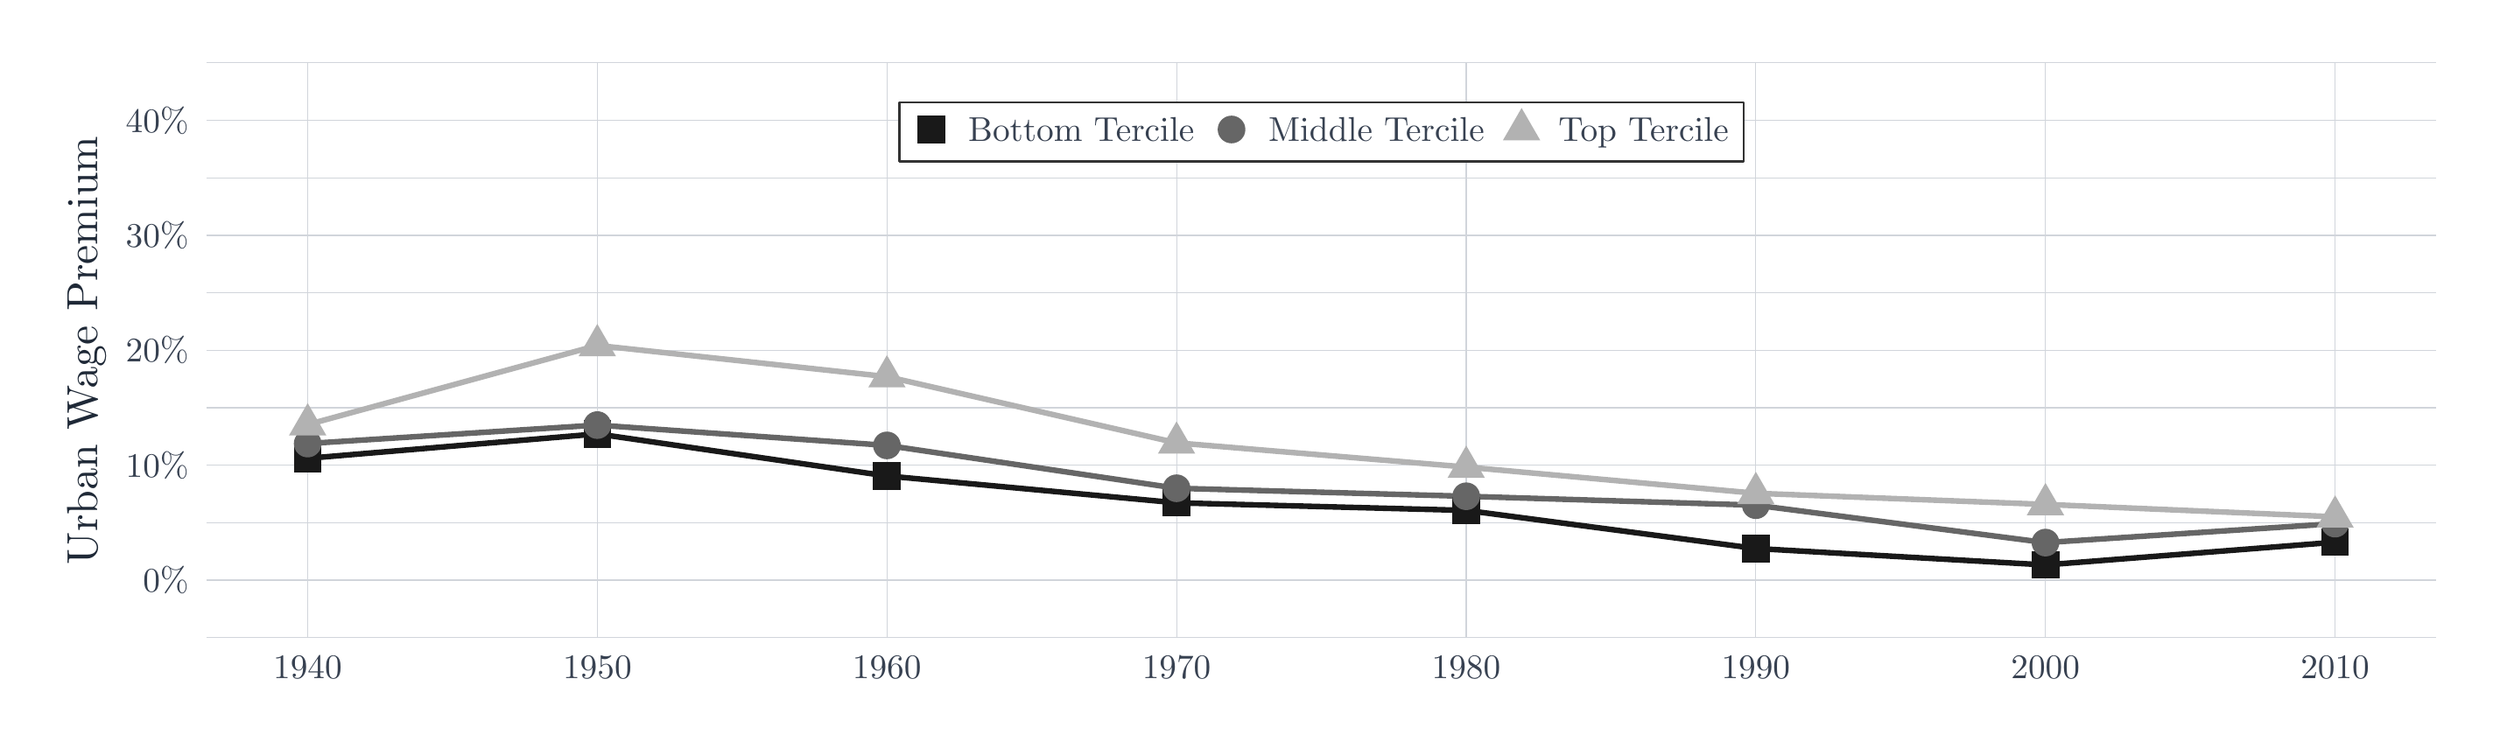
\begin{tikzpicture}[x=1pt,y=1pt]
\definecolor{fillColor}{RGB}{255,255,255}
\path[use as bounding box,fill=fillColor] (0,0) rectangle (1011.78,289.08);
\begin{scope}
\path[clip] (  0.00,  0.00) rectangle (1011.78,289.08);
\definecolor{drawColor}{RGB}{255,255,255}

\path[draw=drawColor,line width= 0.8pt,line join=round,line cap=round,fill=fillColor] (  0.00,  0.00) rectangle (1011.78,289.08);
\end{scope}
\begin{scope}
\path[clip] ( 75.16, 35.76) rectangle (995.78,273.08);
\definecolor{drawColor}{RGB}{255,255,255}
\definecolor{fillColor}{RGB}{255,255,255}

\path[draw=drawColor,line width= 0.8pt,line join=round,line cap=round,fill=fillColor] ( 75.16, 35.76) rectangle (995.78,273.08);
\definecolor{drawColor}{RGB}{209,213,219}

\path[draw=drawColor,line width= 0.4pt,line join=round] ( 75.16, 35.76) --
	(995.78, 35.76);

\path[draw=drawColor,line width= 0.4pt,line join=round] ( 75.16, 83.22) --
	(995.78, 83.22);

\path[draw=drawColor,line width= 0.4pt,line join=round] ( 75.16,130.69) --
	(995.78,130.69);

\path[draw=drawColor,line width= 0.4pt,line join=round] ( 75.16,178.15) --
	(995.78,178.15);

\path[draw=drawColor,line width= 0.4pt,line join=round] ( 75.16,225.62) --
	(995.78,225.62);

\path[draw=drawColor,line width= 0.4pt,line join=round] ( 75.16,273.08) --
	(995.78,273.08);

\path[draw=drawColor,line width= 0.4pt,line join=round] ( 75.16, 59.49) --
	(995.78, 59.49);

\path[draw=drawColor,line width= 0.4pt,line join=round] ( 75.16,106.95) --
	(995.78,106.95);

\path[draw=drawColor,line width= 0.4pt,line join=round] ( 75.16,154.42) --
	(995.78,154.42);

\path[draw=drawColor,line width= 0.4pt,line join=round] ( 75.16,201.88) --
	(995.78,201.88);

\path[draw=drawColor,line width= 0.4pt,line join=round] ( 75.16,249.35) --
	(995.78,249.35);

\path[draw=drawColor,line width= 0.4pt,line join=round] (117.01, 35.76) --
	(117.01,273.08);

\path[draw=drawColor,line width= 0.4pt,line join=round] (236.57, 35.76) --
	(236.57,273.08);

\path[draw=drawColor,line width= 0.4pt,line join=round] (356.13, 35.76) --
	(356.13,273.08);

\path[draw=drawColor,line width= 0.4pt,line join=round] (475.69, 35.76) --
	(475.69,273.08);

\path[draw=drawColor,line width= 0.4pt,line join=round] (595.25, 35.76) --
	(595.25,273.08);

\path[draw=drawColor,line width= 0.4pt,line join=round] (714.81, 35.76) --
	(714.81,273.08);

\path[draw=drawColor,line width= 0.4pt,line join=round] (834.37, 35.76) --
	(834.37,273.08);

\path[draw=drawColor,line width= 0.4pt,line join=round] (953.93, 35.76) --
	(953.93,273.08);
\definecolor{drawColor}{gray}{0.10}

\path[draw=drawColor,line width= 2.3pt,line join=round] (117.01,109.80) --
	(236.57,119.89) --
	(356.13,102.52) --
	(475.69, 91.43) --
	(595.25, 88.30) --
	(714.81, 72.56) --
	(834.37, 65.78) --
	(953.93, 75.16);
\definecolor{drawColor}{gray}{0.40}

\path[draw=drawColor,line width= 2.3pt,line join=round] (117.01,115.90) --
	(236.57,123.53) --
	(356.13,115.14) --
	(475.69, 97.44) --
	(595.25, 94.13) --
	(714.81, 90.45) --
	(834.37, 75.00) --
	(953.93, 82.83);
\definecolor{drawColor}{gray}{0.70}

\path[draw=drawColor,line width= 2.3pt,line join=round] (117.01,123.73) --
	(236.57,156.42) --
	(356.13,143.54) --
	(475.69,116.19) --
	(595.25,106.20) --
	(714.81, 95.37) --
	(834.37, 90.77) --
	(953.93, 85.66);
\definecolor{fillColor}{gray}{0.10}

\path[fill=fillColor] (111.30,104.09) --
	(122.72,104.09) --
	(122.72,115.51) --
	(111.30,115.51) --
	cycle;
\definecolor{fillColor}{gray}{0.40}

\path[fill=fillColor] (117.01,115.90) circle (  5.71);
\definecolor{fillColor}{gray}{0.70}

\path[fill=fillColor] (117.01,132.61) --
	(124.70,119.29) --
	(109.32,119.29) --
	cycle;
\definecolor{fillColor}{gray}{0.10}

\path[fill=fillColor] (230.86,114.18) --
	(242.28,114.18) --
	(242.28,125.60) --
	(230.86,125.60) --
	cycle;
\definecolor{fillColor}{gray}{0.40}

\path[fill=fillColor] (236.57,123.53) circle (  5.71);
\definecolor{fillColor}{gray}{0.70}

\path[fill=fillColor] (236.57,165.30) --
	(244.26,151.98) --
	(228.88,151.98) --
	cycle;
\definecolor{fillColor}{gray}{0.10}

\path[fill=fillColor] (350.42, 96.81) --
	(361.84, 96.81) --
	(361.84,108.23) --
	(350.42,108.23) --
	cycle;
\definecolor{fillColor}{gray}{0.40}

\path[fill=fillColor] (356.13,115.14) circle (  5.71);
\definecolor{fillColor}{gray}{0.70}

\path[fill=fillColor] (356.13,152.42) --
	(363.82,139.10) --
	(348.44,139.10) --
	cycle;
\definecolor{fillColor}{gray}{0.10}

\path[fill=fillColor] (469.98, 85.72) --
	(481.40, 85.72) --
	(481.40, 97.14) --
	(469.98, 97.14) --
	cycle;
\definecolor{fillColor}{gray}{0.40}

\path[fill=fillColor] (475.69, 97.44) circle (  5.71);
\definecolor{fillColor}{gray}{0.70}

\path[fill=fillColor] (475.69,125.07) --
	(483.38,111.75) --
	(468.00,111.75) --
	cycle;
\definecolor{fillColor}{gray}{0.10}

\path[fill=fillColor] (589.54, 82.59) --
	(600.96, 82.59) --
	(600.96, 94.01) --
	(589.54, 94.01) --
	cycle;
\definecolor{fillColor}{gray}{0.40}

\path[fill=fillColor] (595.25, 94.13) circle (  5.71);
\definecolor{fillColor}{gray}{0.70}

\path[fill=fillColor] (595.25,115.08) --
	(602.94,101.76) --
	(587.56,101.76) --
	cycle;
\definecolor{fillColor}{gray}{0.10}

\path[fill=fillColor] (709.10, 66.85) --
	(720.52, 66.85) --
	(720.52, 78.27) --
	(709.10, 78.27) --
	cycle;
\definecolor{fillColor}{gray}{0.40}

\path[fill=fillColor] (714.81, 90.45) circle (  5.71);
\definecolor{fillColor}{gray}{0.70}

\path[fill=fillColor] (714.81,104.25) --
	(722.50, 90.93) --
	(707.12, 90.93) --
	cycle;
\definecolor{fillColor}{gray}{0.10}

\path[fill=fillColor] (828.66, 60.07) --
	(840.08, 60.07) --
	(840.08, 71.49) --
	(828.66, 71.49) --
	cycle;
\definecolor{fillColor}{gray}{0.40}

\path[fill=fillColor] (834.37, 75.00) circle (  5.71);
\definecolor{fillColor}{gray}{0.70}

\path[fill=fillColor] (834.37, 99.65) --
	(842.06, 86.33) --
	(826.68, 86.33) --
	cycle;
\definecolor{fillColor}{gray}{0.10}

\path[fill=fillColor] (948.22, 69.45) --
	(959.64, 69.45) --
	(959.64, 80.87) --
	(948.22, 80.87) --
	cycle;
\definecolor{fillColor}{gray}{0.40}

\path[fill=fillColor] (953.93, 82.83) circle (  5.71);
\definecolor{fillColor}{gray}{0.70}

\path[fill=fillColor] (953.93, 94.54) --
	(961.62, 81.22) --
	(946.24, 81.22) --
	cycle;
\end{scope}
\begin{scope}
\path[clip] (  0.00,  0.00) rectangle (1011.78,289.08);
\definecolor{drawColor}{RGB}{55,65,81}

\node[text=drawColor,anchor=base east,inner sep=0pt, outer sep=0pt, scale=  1.42] at ( 67.96, 54.59) {0\%};

\node[text=drawColor,anchor=base east,inner sep=0pt, outer sep=0pt, scale=  1.42] at ( 67.96,102.06) {10\%};

\node[text=drawColor,anchor=base east,inner sep=0pt, outer sep=0pt, scale=  1.42] at ( 67.96,149.52) {20\%};

\node[text=drawColor,anchor=base east,inner sep=0pt, outer sep=0pt, scale=  1.42] at ( 67.96,196.99) {30\%};

\node[text=drawColor,anchor=base east,inner sep=0pt, outer sep=0pt, scale=  1.42] at ( 67.96,244.45) {40\%};
\end{scope}
\begin{scope}
\path[clip] (  0.00,  0.00) rectangle (1011.78,289.08);
\definecolor{drawColor}{RGB}{55,65,81}

\node[text=drawColor,anchor=base,inner sep=0pt, outer sep=0pt, scale=  1.42] at (117.01, 18.76) {1940};

\node[text=drawColor,anchor=base,inner sep=0pt, outer sep=0pt, scale=  1.42] at (236.57, 18.76) {1950};

\node[text=drawColor,anchor=base,inner sep=0pt, outer sep=0pt, scale=  1.42] at (356.13, 18.76) {1960};

\node[text=drawColor,anchor=base,inner sep=0pt, outer sep=0pt, scale=  1.42] at (475.69, 18.76) {1970};

\node[text=drawColor,anchor=base,inner sep=0pt, outer sep=0pt, scale=  1.42] at (595.25, 18.76) {1980};

\node[text=drawColor,anchor=base,inner sep=0pt, outer sep=0pt, scale=  1.42] at (714.81, 18.76) {1990};

\node[text=drawColor,anchor=base,inner sep=0pt, outer sep=0pt, scale=  1.42] at (834.37, 18.76) {2000};

\node[text=drawColor,anchor=base,inner sep=0pt, outer sep=0pt, scale=  1.42] at (953.93, 18.76) {2010};
\end{scope}
\begin{scope}
\path[clip] (  0.00,  0.00) rectangle (1011.78,289.08);
\definecolor{drawColor}{RGB}{31,41,55}

\node[text=drawColor,rotate= 90.00,anchor=base,inner sep=0pt, outer sep=0pt, scale=  1.80] at ( 30.15,154.42) {Urban Wage Premium};
\end{scope}
\begin{scope}
\path[clip] (  0.00,  0.00) rectangle (1011.78,289.08);
\definecolor{drawColor}{gray}{0.20}
\definecolor{fillColor}{RGB}{255,255,255}

\path[draw=drawColor,line width= 0.8pt,line join=round,line cap=round,fill=fillColor] (361.26,232.37) rectangle (709.68,256.83);
\end{scope}
\begin{scope}
\path[clip] (  0.00,  0.00) rectangle (1011.78,289.08);
\definecolor{drawColor}{RGB}{255,255,255}
\definecolor{fillColor}{RGB}{255,255,255}

\path[draw=drawColor,line width= 0.8pt,line join=round,line cap=round,fill=fillColor] (367.26,238.37) rectangle (381.72,252.83);
\end{scope}
\begin{scope}
\path[clip] (  0.00,  0.00) rectangle (1011.78,289.08);
\definecolor{fillColor}{gray}{0.10}

\path[fill=fillColor] (368.78,239.89) --
	(380.20,239.89) --
	(380.20,251.31) --
	(368.78,251.31) --
	cycle;
\end{scope}
\begin{scope}
\path[clip] (  0.00,  0.00) rectangle (1011.78,289.08);
\definecolor{drawColor}{RGB}{255,255,255}
\definecolor{fillColor}{RGB}{255,255,255}

\path[draw=drawColor,line width= 0.8pt,line join=round,line cap=round,fill=fillColor] (491.15,238.37) rectangle (505.60,252.83);
\end{scope}
\begin{scope}
\path[clip] (  0.00,  0.00) rectangle (1011.78,289.08);
\definecolor{fillColor}{gray}{0.40}

\path[fill=fillColor] (498.38,245.60) circle (  5.71);
\end{scope}
\begin{scope}
\path[clip] (  0.00,  0.00) rectangle (1011.78,289.08);
\definecolor{drawColor}{RGB}{255,255,255}
\definecolor{fillColor}{RGB}{255,255,255}

\path[draw=drawColor,line width= 0.8pt,line join=round,line cap=round,fill=fillColor] (610.89,238.37) rectangle (625.35,252.83);
\end{scope}
\begin{scope}
\path[clip] (  0.00,  0.00) rectangle (1011.78,289.08);
\definecolor{fillColor}{gray}{0.70}

\path[fill=fillColor] (618.12,254.48) --
	(625.81,241.16) --
	(610.43,241.16) --
	cycle;
\end{scope}
\begin{scope}
\path[clip] (  0.00,  0.00) rectangle (1011.78,289.08);
\definecolor{drawColor}{RGB}{55,65,81}

\node[text=drawColor,anchor=base west,inner sep=0pt, outer sep=0pt, scale=  1.42] at (389.72,240.70) {Bottom Tercile};
\end{scope}
\begin{scope}
\path[clip] (  0.00,  0.00) rectangle (1011.78,289.08);
\definecolor{drawColor}{RGB}{55,65,81}

\node[text=drawColor,anchor=base west,inner sep=0pt, outer sep=0pt, scale=  1.42] at (513.60,240.70) {Middle Tercile};
\end{scope}
\begin{scope}
\path[clip] (  0.00,  0.00) rectangle (1011.78,289.08);
\definecolor{drawColor}{RGB}{55,65,81}

\node[text=drawColor,anchor=base west,inner sep=0pt, outer sep=0pt, scale=  1.42] at (633.35,240.70) {Top Tercile};
\end{scope}
\end{tikzpicture}
